\documentclass[11pt,a4paper]{ctexart}
\usepackage[margin=2.4cm]{geometry}
\usepackage{graphicx}
\usepackage{booktabs}
\usepackage{amsmath}
\usepackage{hyperref}

\title{反光焦堆 ROI 局部证据与光学机理补充}
\author{SRTP Project Notes}
\date{2026-06-21}

\begin{document}
\maketitle

\section{新增观察}

本补充报告基于 \texttt{钥匙纹路100um} 真实焦堆，对高亮边缘、普通纹理和暗区三个 ROI 做局部焦向分析。结果显示，高亮边缘 ROI 的近饱和层与 Laplacian/Tenengrad 峰值层重合，而普通纹理和暗区的焦点评价峰出现在更靠后的焦层。这说明同一焦堆内部的反光区域和正常纹理区域具有不同的 focus-response 机制。

\section{ROI 统计}

\begin{table}[htbp]
\centering
\begin{tabular}{lrrrr}
\toprule
ROI & max p99 & max sat. ratio & best Laplacian layer & best Tenengrad layer \\
\midrule
highlight\_edge & 1.0000 & 0.2328 & 2 & 2 \\
ordinary\_texture & 0.2627 & 0.0000 & 18 & 18 \\
dark\_region & 0.2000 & 0.0000 & 19 & 19 \\
\bottomrule
\end{tabular}
\caption{ROI-level brightness and focus-measure statistics for the \texttt{钥匙纹路100um} focal stack.}
\end{table}

\begin{figure}[htbp]
\centering
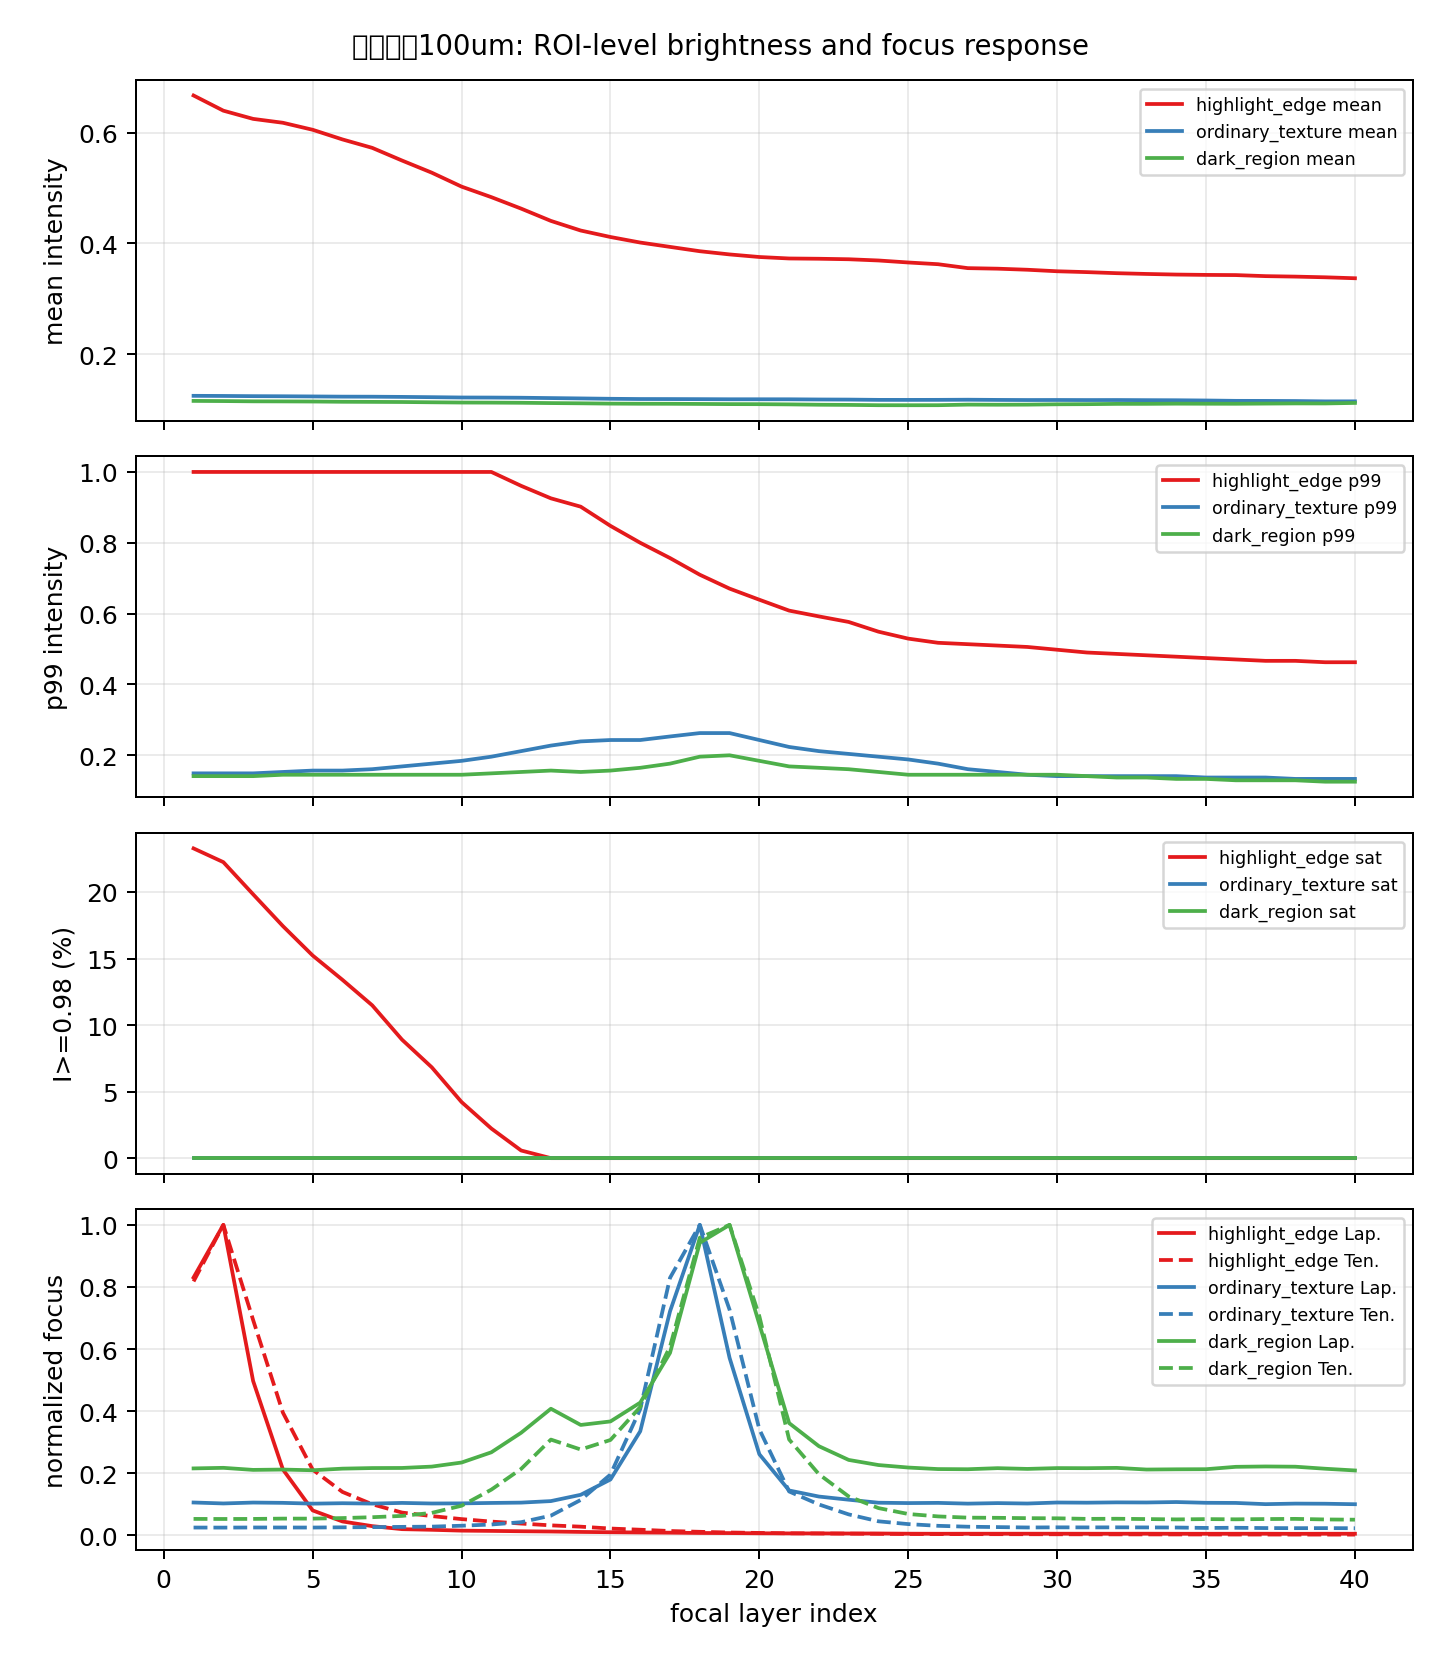
\includegraphics[width=0.95\linewidth]{roi_probe/钥匙纹路100um_roi_curves.png}
\caption{ROI-level brightness, saturation, and focus response. The highlight-edge ROI peaks at glare-dominated early layers, while ordinary and dark ROIs peak around layers 18/19.}
\end{figure}

\begin{figure}[htbp]
\centering
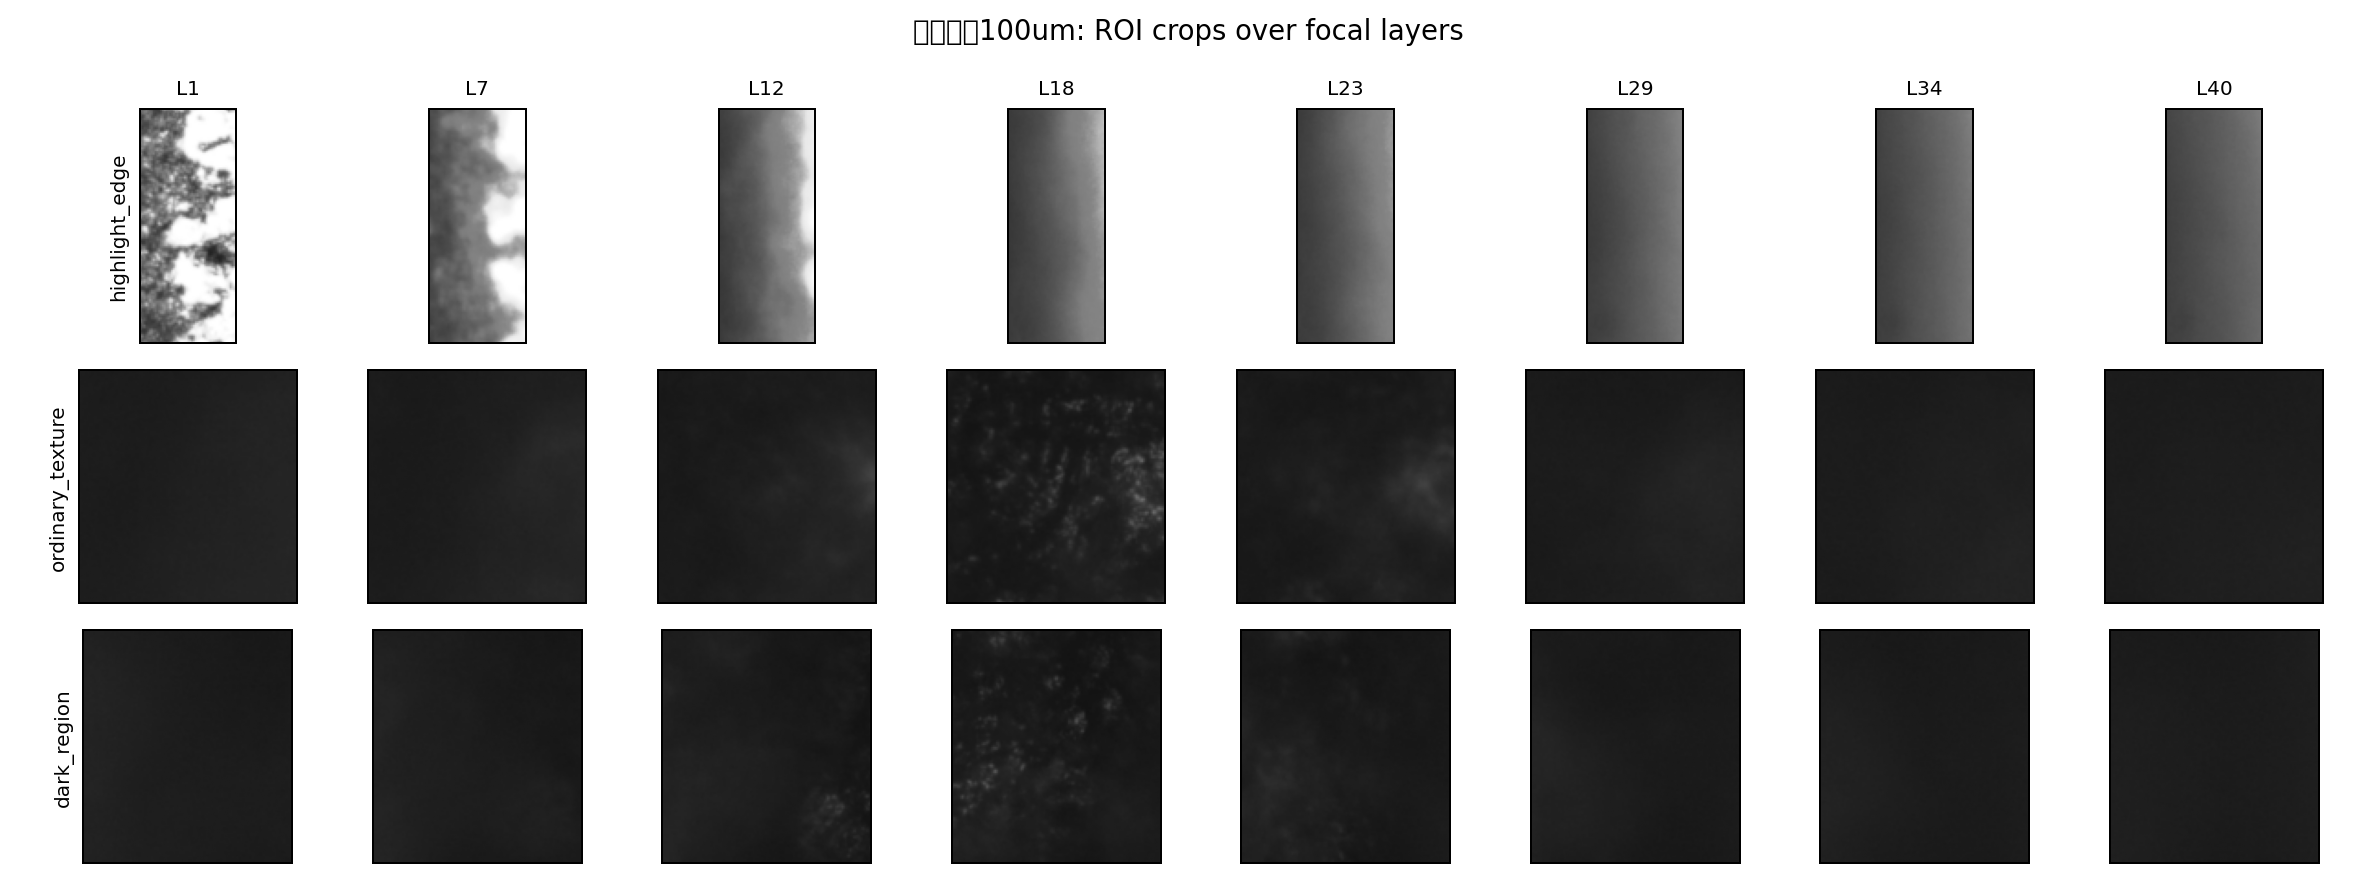
\includegraphics[width=0.95\linewidth]{roi_probe/钥匙纹路100um_roi_montage.png}
\caption{ROI crops over selected focal layers. The highlight-edge ROI shows strong near-saturated structures in early layers, while normal regions become textured around later focal layers.}
\end{figure}

\section{光学解释}

显微物镜 numerical aperture 可写为
\begin{equation}
\mathrm{NA}=n\sin\theta,
\end{equation}
其中 $n$ 为介质折射率，$\theta$ 为接收光锥半角。空气中若 $\mathrm{NA}=0.4$，则 $\theta\approx23.6^\circ$。

设局部法线为 $\mathbf{n}$，入射方向为 $\mathbf{l}$，观察方向为 $\mathbf{v}$，镜面反射方向可写为
\begin{equation}
\mathbf{r}=2(\mathbf{n}\cdot\mathbf{l})\mathbf{n}-\mathbf{l}.
\end{equation}
若
\begin{equation}
\arccos(\mathbf{r}\cdot\mathbf{v}) \leq \arcsin(\mathrm{NA}/n_{\mathrm{medium}}),
\end{equation}
则该局部微表面更可能将反射光送入物镜接收锥并形成高亮。

传统 DFF 的焦点评价函数可抽象为
\begin{equation}
F_k(\mathbf{x})=\Phi(I_k(\Omega_\mathbf{x})).
\end{equation}
当局部高亮或近饱和区域在离焦状态下形成强边缘，$\Phi$ 可能在反光层达到峰值，导致 $\arg\max_k F_k(\mathbf{x})$ 偏离真实几何焦层。

\section{论文写作建议}

可将本补充结果写入 failure-analysis 段落：

\begin{quote}
In the key-texture focal stack, the highlight-edge ROI reaches a near-saturation ratio of 23.28\%, with both Laplacian and Tenengrad responses peaking at focal layer 2. In contrast, ordinary-texture and dark-region ROIs contain no near-saturated pixels and peak at layers 18/19. This ROI-level discrepancy indicates that glare-dominated regions can produce focus-measure peaks unrelated to normal texture sharpness, motivating explicit glare-risk and saturation-persistence priors.
\end{quote}

\section{References}

\begin{itemize}
\item Nikon MicroscopyU, Numerical Aperture. \url{https://www.microscopyu.com/microscopy-basics/numerical-aperture}
\item Cook and Torrance, A Reflectance Model for Computer Graphics. \url{https://doi.org/10.1145/357290.357293}
\item Nayar and Nakagawa, Shape from Focus. \url{https://doi.org/10.1109/34.308479}
\item Yang et al., Deep Depth from Focus with Differential Focus Volume. \url{https://arxiv.org/abs/2112.01712}
\item Fujimura et al., Deep Depth from Focal Stack with Defocus Model for Camera-Setting Invariance. \url{https://arxiv.org/abs/2202.13055}
\end{itemize}

\end{document}
